\documentclass[conference]{IEEEtran}
\usepackage{amsmath,amssymb}
\usepackage{booktabs}
\usepackage{graphicx}
\usepackage{pgfplots}
\usepgfplotslibrary{groupplots}
\pgfplotsset{compat=1.18}
\usepackage{hyperref}

% All figures are drawn with pgfplots from numbers in this file, so the paper
% compiles on its own with no external image files. Every number is traceable
% to the telemetry named in Section~\ref{sec:repro}.

\renewcommand{\topfraction}{0.9}
\renewcommand{\bottomfraction}{0.9}
\renewcommand{\textfraction}{0.07}
\renewcommand{\floatpagefraction}{0.7}
\renewcommand{\dbltopfraction}{0.9}
\renewcommand{\dblfloatpagefraction}{0.7}

\definecolor{kfive}{HTML}{2563EB}
\definecolor{eaglethree}{HTML}{F59E0B}
\definecolor{othergrey}{HTML}{9CA3AF}

\begin{document}

\title{Fixed-Window Draft-Model Speculative Decoding \\ versus EAGLE-3:
A Like-for-Like, Energy-Measured Comparison \\ in vLLM and SGLang}

\author{
\IEEEauthorblockN{Zanno Jacklin}
\IEEEauthorblockA{Independent Researcher, Creepybits}
}

\maketitle

\begin{abstract}
Speculative decoding with a separate small draft model is a well-established
technique, shipped today in vLLM, SGLang and Hugging Face Transformers. Newer
methods such as EAGLE-3 replace the draft model with a lightweight draft head
trained for one specific target model. We compare a fixed-window draft-model
configuration (``K5'': Llama-3.2-1B drafting $K{=}5$ tokens for
Llama-3.1-8B) against EAGLE-3, EAGLE-1 and n-gram drafting, measuring
throughput and GPU energy per token. The comparison is like-for-like: each
method runs inside the same engine as its competitors, each method is given
several configurations, the best configuration is chosen on half of 27
prompts and reported on the other half, and every run executes in a fresh
process bracketed by baseline runs. At batch size~1 on an RTX~5090, K5
increases throughput by +79\% (SGLang) and +60\% (vLLM) and reduces energy
per token by 55\% and 53\% relative to non-speculative decoding. The best
EAGLE-3 configuration is faster in both engines, by 14\% and 8\%
respectively; on energy per token the result is split (K5 uses 10\% more in
SGLang and 9\% less in vLLM). K5 thus attains roughly three quarters to four
fifths of EAGLE-3's throughput gain with comparable energy savings, without
requiring a target-specific trained draft head. We also report that every
speculative method tested diverges from its own engine's non-speculative
output on most prompts in bf16, and that a controlled, cache-free
reimplementation reproduces the mechanism's speed and energy scaling with
acceptance rate at 100\% token fidelity.
\end{abstract}

\begin{IEEEkeywords}
speculative decoding, EAGLE-3, energy-efficient inference, large language models, GPU power measurement, benchmarking methodology
\end{IEEEkeywords}

\section{Introduction}

Autoregressive decoding produces one token per full forward pass of the
target model, leaving much of a modern GPU's parallel capacity unused at
small batch sizes. Speculative decoding~\cite{leviathan2023fast,chen2023accelerating}
lets a cheaper drafter propose several tokens that the target model then
verifies in a single forward pass, keeping the longest prefix that matches
the target's own choice. With greedy decoding the accepted output is, in
exact arithmetic, identical to what the target alone would produce.

The original formulation uses a separate small \emph{draft model} from the
same family. This is not a new technique: it is available as
\texttt{draft\_model} in vLLM~\cite{kwon2023vllm}, as \texttt{STANDALONE} in
SGLang~\cite{zheng2024sglang}, and as assisted generation in Hugging Face
Transformers~\cite{gante2023assisted}. Later methods replace the draft model
with a lightweight head trained on the target model's internal features,
most recently EAGLE-3~\cite{li2024eagle,li2025eagle3}, which is widely
regarded as the stronger approach.

This paper asks a narrow practical question: \emph{inside production serving
engines, how does a simple fixed-window draft-model configuration compare
with EAGLE-3 on both speed and energy?} Our contribution is measurement, not
a new algorithm: (i) a like-for-like benchmarking protocol designed so that
no method is handicapped by configuration choice, run order, cross-request
memory or engine differences (Section~\ref{sec:protocol}); (ii) results in
two engines, including GPU energy per token (Section~\ref{sec:results});
and (iii) a controlled, cache-free reimplementation that isolates the
mechanism's behaviour (Section~\ref{sec:isolation}).

\subsection{Related work}

Beyond draft models and EAGLE, adaptive methods vary the draft length at run
time; AdaEDL~\cite{adaedl2024}, for example, stops drafting early using an
entropy-based bound on acceptance probability and reports 10--57\%
improvement over static draft lengths. This paper keeps the draft length
fixed. An entropy-gated adaptive variant was explored separately in the
parent project and has not, so far, outperformed the fixed window in
single-request testing; we make no claims about it here.

\section{Setup and like-for-like protocol}
\label{sec:protocol}

\subsection{Models, hardware and software}

Target: Llama-3.1-8B-Instruct. Draft model: Llama-3.2-1B-Instruct. EAGLE
checkpoints: the public EAGLE-1 and EAGLE-3 heads for Llama-3.1-8B-Instruct.
All models in bfloat16, greedy decoding, batch size~1, up to 250 generated
tokens per request with natural end-of-sequence, prompts formatted with the
target's chat template. One NVIDIA RTX~5090 (Blackwell) under WSL2, without
clock locking. Engines: vLLM~0.27.1 and SGLang~0.5.20, each in its own
Python environment (PyTorch~2.13).

\subsection{Energy measurement}

GPU energy is read from the on-board hardware energy counter
(\texttt{nvmlDeviceGetTotalEnergyConsumption}) at the start and end of each
timed request and divided by the number of tokens produced. Power and
temperature are sampled at 100~Hz for warmup and drift diagnostics.

\subsection{Protocol}

\emph{Same engine only.} Methods are compared only within one engine;
numbers from vLLM and SGLang are never placed against each other, since they
differ by engineering rather than algorithm.

\emph{Several configurations per method.} vLLM: draft model with
$K\in\{3,5,7\}$, EAGLE-3 with $K\in\{2,3,5\}$, EAGLE-1 with $K\in\{3,5\}$,
n-gram with $K{=}5$. SGLang: draft model with $K\in\{3,5,7\}$ (chain),
EAGLE-3 with $K\in\{3,5\}$ (chain) and one tree configuration (5 steps,
top-$k$~8, 32 draft tokens), EAGLE-1 with $K{=}5$, n-gram with 16 draft
tokens. K5 is the draft model at $K{=}5$.

\emph{Tuning separated from evaluation.} 27 prompts are used: the project's
three reference prompts (a poem, a physics explanation, a code task) plus
24 original prompts, three in each of the eight categories used by
MT-Bench~\cite{zheng2023judging} (not the MT-Bench questions themselves).
Each method's best configuration is selected on 14 prompts and reported on
the remaining 13 (alternating within category), so methods with more
configurations do not gain from selecting and grading on the same data.

\emph{No repeated exposure.} Each configuration runs in a fresh engine
process, and each timed prompt is generated exactly once per process.
Repetition (two per configuration) happens across processes. This prevents
methods that keep memory across requests from drafting their own previous
answer to an identical greedy prompt. Warmup uses separate prompts that are
never timed, and prefix caching is disabled in both engines.

\emph{Drift control.} Each engine block starts and ends with a baseline run
(no speculation). Speedups are computed per prompt against the mean of the
two baselines of the same block. Configuration order is randomized per
repetition (seed recorded) and engine order alternates. Each run first
warms the GPU in a closed loop until per-prompt power and temperature stop
drifting (minimum 150~s), and a short untimed generation on a warmup prompt
precedes every timed request.

\emph{Statistics.} Per-prompt speedups are combined with a geometric mean;
95\% ranges are bootstrap intervals over prompts (2000 resamples).

\emph{Sanity checks.} A configuration is shown but excluded from ``best''
if its mean accept length (tokens per verification step) is below 1.05, if
its speedup exceeds its accept length (impossible, since each verification
step costs at least one ordinary decoding step), or if output lengths
differ from baseline on more than 20\% of prompts.

\emph{Known engine asymmetry.} vLLM~0.27.1 runs \texttt{draft\_model} on its
older V1 model runner with asynchronous scheduling disabled, while EAGLE-3
runs on the V2 model runner with asynchronous scheduling enabled (both
confirmed from vLLM's own logs). We additionally ran EAGLE-3 with
asynchronous scheduling disabled (``EAGLE-3, async off''); the model-runner
difference could not be matched.

\section{Results}
\label{sec:results}

\begin{figure*}[!t]
\centering
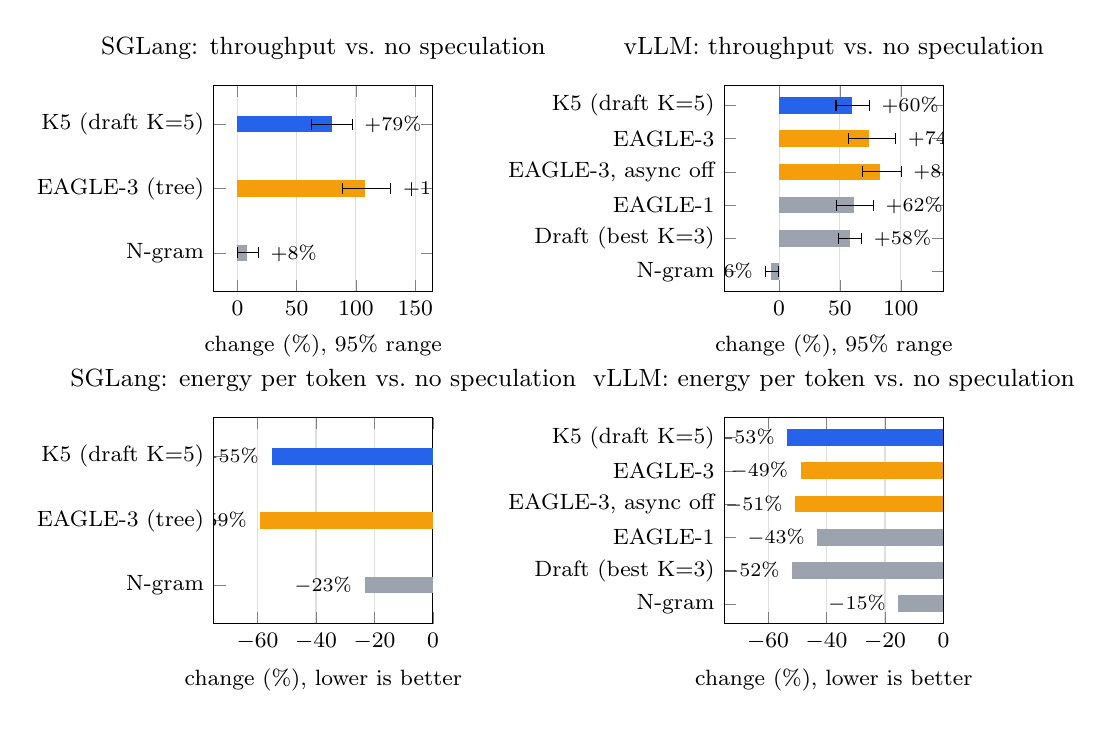
\begin{tikzpicture}
\begin{groupplot}[
  group style={group size=2 by 2, horizontal sep=3.7cm, vertical sep=1.6cm},
  width=0.36\textwidth, height=4.2cm,
  /pgf/bar width=6pt, /pgf/bar shift=0pt,
  y dir=reverse,
  tick label style={font=\footnotesize},
  label style={font=\footnotesize},
  title style={font=\small},
  xmajorgrids, grid style={gray!25},
  error bars/x dir=both, error bars/x explicit,
]
% ---- SGLang speed (evaluation prompts) ----
\nextgroupplot[title={SGLang: throughput vs.\ no speculation}, xlabel={change (\%), 95\% range},
  xmin=-20, xmax=165, ymin=0.4, ymax=3.6,
  ytick={1,2,3}, yticklabels={K5 (draft K=5), EAGLE-3 (tree), N-gram}]
\addplot[xbar, fill=kfive, draw=none, error bars/error bar style={black}] coordinates {(79.4,1) += (17.4,0) -= (16.6,0)};
\node[font=\scriptsize, anchor=west] at (axis cs:98.8,1) {+79\%};
\addplot[xbar, fill=eaglethree, draw=none, error bars/error bar style={black}] coordinates {(107.5,2) += (22.0,0) -= (19.0,0)};
\node[font=\scriptsize, anchor=west] at (axis cs:131.5,2) {+108\%};
\addplot[xbar, fill=othergrey, draw=none, error bars/error bar style={black}] coordinates {(8.1,3) += (9.7,0) -= (8.1,0)};
\node[font=\scriptsize, anchor=west] at (axis cs:19.8,3) {+8\%};
% ---- vLLM speed ----
\nextgroupplot[title={vLLM: throughput vs.\ no speculation}, xlabel={change (\%), 95\% range},
  xmin=-45, xmax=135, ymin=0.4, ymax=6.6,
  ytick={1,2,3,4,5,6}, yticklabels={K5 (draft K=5), EAGLE-3, {EAGLE-3, async off}, EAGLE-1, Draft (best K=3), N-gram}]
\addplot[xbar, fill=kfive, draw=none, error bars/error bar style={black}] coordinates {(59.9,1) += (14.2,0) -= (13.1,0)};
\node[font=\scriptsize, anchor=west] at (axis cs:76.1,1) {+60\%};
\addplot[xbar, fill=eaglethree, draw=none, error bars/error bar style={black}] coordinates {(74.2,2) += (21.5,0) -= (17.1,0)};
\node[font=\scriptsize, anchor=west] at (axis cs:97.7,2) {+74\%};
\addplot[xbar, fill=eaglethree, draw=none, error bars/error bar style={black}] coordinates {(83.2,3) += (17.1,0) -= (14.8,0)};
\node[font=\scriptsize, anchor=west] at (axis cs:102.3,3) {+83\%};
\addplot[xbar, fill=othergrey, draw=none, error bars/error bar style={black}] coordinates {(61.5,4) += (16.0,0) -= (14.2,0)};
\node[font=\scriptsize, anchor=west] at (axis cs:79.5,4) {+62\%};
\addplot[xbar, fill=othergrey, draw=none, error bars/error bar style={black}] coordinates {(58.3,5) += (9.6,0) -= (9.4,0)};
\node[font=\scriptsize, anchor=west] at (axis cs:69.9,5) {+58\%};
\addplot[xbar, fill=othergrey, draw=none, error bars/error bar style={black}] coordinates {(-6.4,6) += (5.6,0) -= (5.1,0)};
\node[font=\scriptsize, anchor=east] at (axis cs:-13.5,6) {$-$6\%};
% ---- SGLang energy ----
\nextgroupplot[title={SGLang: energy per token vs.\ no speculation}, xlabel={change (\%), lower is better},
  xmin=-75, xmax=0, ymin=0.4, ymax=3.6,
  ytick={1,2,3}, yticklabels={K5 (draft K=5), EAGLE-3 (tree), N-gram}]
\addplot[xbar, fill=kfive, draw=none] coordinates {(-55.2,1)};
\node[font=\scriptsize, anchor=east] at (axis cs:-56.2,1) {$-$55\%};
\addplot[xbar, fill=eaglethree, draw=none] coordinates {(-59.3,2)};
\node[font=\scriptsize, anchor=east] at (axis cs:-60.3,2) {$-$59\%};
\addplot[xbar, fill=othergrey, draw=none] coordinates {(-23.4,3)};
\node[font=\scriptsize, anchor=east] at (axis cs:-24.4,3) {$-$23\%};
% ---- vLLM energy ----
\nextgroupplot[title={vLLM: energy per token vs.\ no speculation}, xlabel={change (\%), lower is better},
  xmin=-75, xmax=0, ymin=0.4, ymax=6.6,
  ytick={1,2,3,4,5,6}, yticklabels={K5 (draft K=5), EAGLE-3, {EAGLE-3, async off}, EAGLE-1, Draft (best K=3), N-gram}]
\addplot[xbar, fill=kfive, draw=none] coordinates {(-53.4,1)};
\node[font=\scriptsize, anchor=east] at (axis cs:-54.4,1) {$-$53\%};
\addplot[xbar, fill=eaglethree, draw=none] coordinates {(-48.8,2)};
\node[font=\scriptsize, anchor=east] at (axis cs:-49.8,2) {$-$49\%};
\addplot[xbar, fill=eaglethree, draw=none] coordinates {(-50.7,3)};
\node[font=\scriptsize, anchor=east] at (axis cs:-51.7,3) {$-$51\%};
\addplot[xbar, fill=othergrey, draw=none] coordinates {(-43.1,4)};
\node[font=\scriptsize, anchor=east] at (axis cs:-44.1,4) {$-$43\%};
\addplot[xbar, fill=othergrey, draw=none] coordinates {(-51.7,5)};
\node[font=\scriptsize, anchor=east] at (axis cs:-52.7,5) {$-$52\%};
\addplot[xbar, fill=othergrey, draw=none] coordinates {(-15.4,6)};
\node[font=\scriptsize, anchor=east] at (axis cs:-16.4,6) {$-$15\%};
\end{groupplot}
\end{tikzpicture}
\caption{Like-for-like comparison: each method at its best configuration
(chosen on 14 prompts), reported on the 13 evaluation prompts. Batch size~1,
RTX~5090. Error bars: 95\% bootstrap range over prompts. Engines are shown
separately and are not comparable with each other. SGLang's EAGLE-1 is
omitted (it failed the sanity check; Section~\ref{sec:results-other}).}
\label{fig:likeforlike}
\end{figure*}

\subsection{K5 versus each method's best configuration}

Figure~\ref{fig:likeforlike} and Table~\ref{tab:h2h} summarise the
comparison on the evaluation prompts. All 46 runs completed; baseline
drift within a block (closing versus opening baseline) was 1.5\% in SGLang
and 4.1\% in vLLM, the latter above our 3\% warning threshold, so small
vLLM differences should be read with caution.

\begin{table}[t]
\centering
\caption{K5 relative to the best configuration of each other method
(evaluation prompts, 13). Speed: positive means K5 is faster. Energy:
negative means K5 uses less energy per token.}
\label{tab:h2h}
\setlength{\tabcolsep}{3pt}
\resizebox{\linewidth}{!}{%
\begin{tabular}{llccc}
\toprule
Engine & Opponent (best config) & K5 speed [95\%] & K5 faster & K5 energy \\
\midrule
SGLang & EAGLE-3 (tree) & $-$13.6\% [$-$19.0, $-$8.5] & 0/13 & +10.2\% \\
SGLang & N-gram & +65.9\% [+57.1, +75.2] & 13/13 & $-$41.5\% \\
\midrule
vLLM & EAGLE-3 ($K{=}5$) & $-$8.2\% [$-$14.5, $-$1.5] & 4/13 & $-$9.1\% \\
vLLM & EAGLE-3, async off ($K{=}3$) & $-$12.7\% [$-$17.3, $-$7.2] & 2/13 & $-$5.5\% \\
vLLM & EAGLE-1 ($K{=}3$) & $-$1.0\% [$-$5.3, +3.5] & 7/13 & $-$18.2\% \\
vLLM & N-gram & +70.9\% [+62.5, +79.7] & 13/13 & $-$45.0\% \\
\bottomrule
\end{tabular}}
\end{table}

\textbf{Speed.} The best EAGLE-3 configuration is faster than K5 in both
engines: by 13.6\% in SGLang, where the tree configuration wins, and by
8.2\% in vLLM. In SGLang, EAGLE-3 in chain mode ($K{=}3$ or $5$) is
\emph{slower} than K5 (Table~\ref{tab:all}); only the tree configuration
overtakes it. Measured as a share of the best EAGLE-3's throughput gain
over no speculation, K5 reaches about 74\% in SGLang
($+79.4\%$ vs.\ $+107.5\%$) and 81\% in vLLM ($+59.9\%$ vs.\ $+74.2\%$).
By prompt category (all prompts), EAGLE-3's advantage is smallest on the
math, coding and roleplay prompts and largest on the humanities prompts and
the three reference prompts; in vLLM, K5 is ahead on the math category
($+75.5\%$ vs.\ $+67.1\%$).

\textbf{Energy.} The energy result is split: K5 uses 10.2\% more energy
per token than the best EAGLE-3 in SGLang and 9.1\% less in vLLM. In both
engines K5 roughly halves energy per token relative to non-speculative
decoding ($-55.2\%$ SGLang, $-53.4\%$ vLLM).

\textbf{N-gram and EAGLE-1.} K5 is far faster than n-gram drafting in both
engines, and is statistically indistinguishable from EAGLE-1 in vLLM on
speed while using 18\% less energy per token.

\subsection{Choice of $K$}

The fixed window $K{=}5$ is as good as any window tested for the draft
model. In SGLang it is the best draft configuration; in vLLM the tuning
half selected $K{=}3$, but on the evaluation prompts K5 and $K{=}3$ are
indistinguishable (K5 +1.0\%, 95\% range $-$2.8\% to +4.8\%).

\begin{table*}[t]
\centering
\caption{Every configuration, all 27 prompts, two runs each. Accept length
is the mean number of tokens produced per target verification step.
Fidelity: mean share of each output that matches the same engine's first
baseline run before the first differing token / share of outputs that are
identical. Baseline run versus baseline run: 100\% / 100\% in both engines.}
\label{tab:all}
\resizebox{\textwidth}{!}{%
\begin{tabular}{lcccc@{\hskip 18pt}lcccc}
\toprule
\multicolumn{5}{c}{SGLang 0.5.20} & \multicolumn{5}{c}{vLLM 0.27.1} \\
\cmidrule(r{12pt}){1-5}\cmidrule{6-10}
Config & Speed [95\%] & Energy & Acc.\ len & Fidelity &
Config & Speed [95\%] & Energy & Acc.\ len & Fidelity \\
\midrule
EAGLE-3 tree & +106.8 [+94.7, +119.7] & $-$59.2 & 3.53 & 62 / 41 &
EAGLE-3 $K$3 async off & +79.6 [+70.4, +90.2] & $-$50.1 & 2.21 & 65 / 44 \\
\textbf{K5} & \textbf{+76.7 [+66.1, +88.3]} & $-$54.3 & 4.28 & 52 / 30 &
EAGLE-3 $K$5 async off & +76.1 [+64.0, +89.1] & $-$50.0 & 2.47 & 72 / 48 \\
Draft $K$7 & +74.0 [+60.4, +89.7] & $-$52.9 & 5.07 & 55 / 30 &
EAGLE-3 $K$3 & +74.0 [+64.9, +84.2] & $-$49.4 & 2.21 & 65 / 44 \\
Draft $K$3 & +65.8 [+58.6, +73.2] & $-$51.5 & 3.20 & 58 / 37 &
EAGLE-3 $K$5 & +73.8 [+62.2, +86.1] & $-$48.9 & 2.47 & 72 / 48 \\
EAGLE-3 $K$5 & +55.2 [+45.1, +66.4] & $-$47.7 & 2.46 & 52 / 30 &
EAGLE-3 $K$2 & +65.8 [+59.4, +72.5] & $-$47.3 & 1.99 & 65 / 44 \\
EAGLE-3 $K$3 & +53.8 [+46.5, +62.5] & $-$48.8 & 2.20 & 62 / 41 &
EAGLE-1 $K$3 & +59.7 [+51.4, +68.9] & $-$42.2 & 2.27 & 63 / 37 \\
N-gram (16) & +8.0 [+2.7, +13.8] & $-$23.2 & 1.41 & 52 / 31 &
Draft $K$3 & +56.6 [+50.6, +63.2] & $-$51.3 & 3.18 & 58 / 33 \\
EAGLE-1 $K$5$^\dagger$ & $-$44.1 [$-$44.4, $-$43.9] & +49.2 & 1.01 & 54 / 30 &
\textbf{K5} & \textbf{+54.6 [+45.3, +64.7]} & $-$51.7 & 4.19 & 59 / 33 \\
 & & & & &
Draft $K$7 & +48.7 [+37.1, +61.7] & $-$49.3 & 4.93 & 62 / 33 \\
 & & & & &
EAGLE-1 $K$5 & +45.3 [+35.8, +56.3] & $-$36.4 & 2.43 & 58 / 33 \\
 & & & & &
N-gram $K$5 & $-$7.6 [$-$10.9, $-$4.1] & $-$14.1 & 1.93 & 67 / 48 \\
\bottomrule
\multicolumn{10}{l}{\footnotesize Speed and energy in \% relative to no speculation.
$^\dagger$Failed the sanity check (accept length $\approx$1: drafts almost never accepted); excluded.}
\end{tabular}}
\end{table*}

\subsection{Other observations}
\label{sec:results-other}

\textbf{Broken configurations are caught.} SGLang's EAGLE-1 had an accept
length of 1.01 (drafts almost never accepted) and ran 44\% slower than no
speculation; the sanity check excluded it, consistent with earlier
observations of this configuration. In an earlier, less controlled
benchmark, SGLang's n-gram method had shown implausible throughput (above
900 tokens/s). Under this protocol, where each prompt is seen once per
process, it shows +8\% with an accept length of 1.41. This supports, but
does not prove, the explanation that n-gram drafting previously benefited
from memory of its own earlier answers to repeated identical prompts.

\textbf{Asynchronous scheduling.} Disabling vLLM's asynchronous scheduling
made EAGLE-3 faster, not slower (+79.6\% versus +74.0\% at $K{=}3$, all
prompts). vLLM disabling it for the draft model is therefore not a
handicap to K5 at batch size~1. We do not have an explanation for this.

\textbf{Fidelity in serving engines.} In both engines two non-speculative
baseline runs produce identical output (100\%). Every speculative method,
however, diverges from its engine's baseline at some point in most
responses: on average 52--72\% of each output matches before the first
differing token, and 30--48\% of outputs are fully identical
(Table~\ref{tab:all}). This holds for EAGLE-3 as much as for K5, and even
for SGLang's EAGLE-1, which accepted almost no drafts (54\%). We interpret
this as a numerical effect of running the engines in speculative mode in
bfloat16: verification processes several tokens per forward pass, and the
resulting rounding differences can flip near-tied greedy choices, after
which the texts continue differently. Speculative decoding is lossless in
exact arithmetic; in practice, in these engines, its output should be
expected to differ from non-speculative output after some point, for every
method tested.

\section{Controlled mechanism isolation}
\label{sec:isolation}

Separately from the engine comparison, we reimplemented the fixed-window
draft-verify loop in plain PyTorch/Transformers, with \emph{no} key-value
cache in either arm, so that both arms perform identical full recomputation
and only the mechanism differs. Absolute throughput is therefore far below
a production server; the relative comparison is the result. Three
reference prompts, 10 trials each, closed-loop warmup that converged
(241~s), and residual drift checks with $R^2 \le 0.037$ for every metric.
Output matched the non-speculative baseline token for token on every
prompt (100\% fidelity).

\begin{table}[t]
\centering
\caption{Controlled, cache-free comparison (no KV-cache in either arm).
N=10 trials per prompt, mean $\pm$ s.d.}
\label{tab:isolation}
\setlength{\tabcolsep}{3pt}
\begin{tabular}{lcccccc}
\toprule
Prompt & Base tok/s & Spec.\ tok/s & Speedup & Energy $\Delta$ & Accept \\
\midrule
Poem    & 40.16 $\pm$ 0.28 & 43.55 $\pm$ 0.31 & +8.4\%  & $-$32.7\% & 42.5\% \\
Physics & 40.05 $\pm$ 0.18 & 49.64 $\pm$ 0.43 & +24.0\% & $-$39.2\% & 51.7\% \\
Code    & 40.04 $\pm$ 0.23 & 73.46 $\pm$ 0.74 & +83.5\% & $-$60.8\% & 85.4\% \\
\bottomrule
\end{tabular}
\end{table}

\begin{figure}[t]
\centering
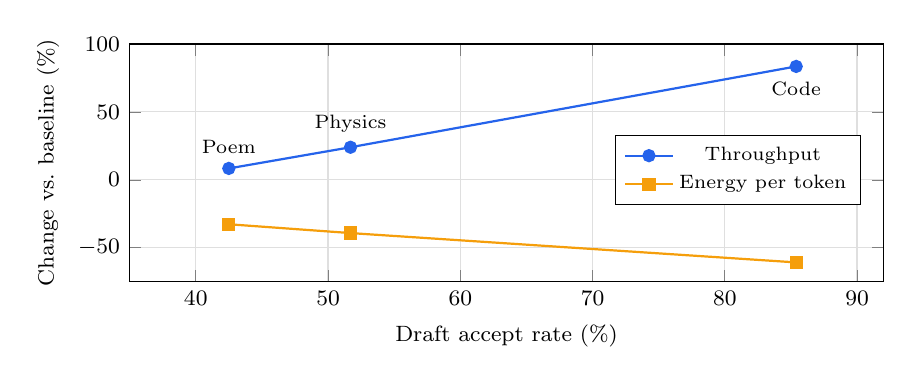
\begin{tikzpicture}
\begin{axis}[
  width=0.92\linewidth, height=4.6cm,
  xlabel={Draft accept rate (\%)}, ylabel={Change vs.\ baseline (\%)},
  xmin=35, xmax=92, ymin=-75, ymax=100,
  label style={font=\footnotesize}, tick label style={font=\footnotesize},
  legend style={font=\scriptsize, at={(0.97,0.47)}, anchor=east},
  xmajorgrids, ymajorgrids, grid style={gray!25},
]
\addplot[color=kfive, mark=*, thick] coordinates {(42.5,8.4) (51.7,24.0) (85.4,83.5)};
\addlegendentry{Throughput}
\addplot[color=eaglethree, mark=square*, thick] coordinates {(42.5,-32.7) (51.7,-39.2) (85.4,-60.8)};
\addlegendentry{Energy per token}
\node[font=\scriptsize, anchor=south] at (axis cs:42.5,12) {Poem};
\node[font=\scriptsize, anchor=south] at (axis cs:51.7,28) {Physics};
\node[font=\scriptsize, anchor=north] at (axis cs:85.4,79) {Code};
\end{axis}
\end{tikzpicture}
\caption{Cache-free comparison: throughput gain and energy reduction both
grow with the draft accept rate, as the mechanism predicts.}
\label{fig:accept}
\end{figure}

Table~\ref{tab:isolation} and Figure~\ref{fig:accept} show the expected
behaviour: gains grow with the draft accept rate, from +8\% on the least
predictable prompt (poetry) to +84\% on code. During speculative decoding
the GPU draws less power (346--364~W versus 463--466~W) despite holding
both models, consistent with fewer full target forward passes per token.
Accept rates in this harness (42.5 / 51.7 / 85.4\%) agree closely with
those measured by vLLM's own independent draft-model implementation on the
same three prompts in an earlier run (43.3 / 57.8 / 85.0\%).

A KV-cached version of this plain Python harness did \emph{not} reproduce a
speedup: speculation was slower than cached baseline decoding on less
predictable prompts. A simple cost model indicates why: in eager Python, a
single forward pass of the 1B draft model costs a large fraction of the 8B
target's per-call time (dominated by per-call overhead rather than
computation), which removes the draft model's advantage. The model's
predictions match the measurements, but per-call times were inferred rather
than measured directly. The practical conclusion is that the mechanism
needs an optimized engine (as in Section~\ref{sec:results}) to pay off with
caching enabled.

\section{Discussion and limitations}

\textbf{What the results support.} Against a properly configured EAGLE-3,
the fixed-window draft model is slower in both engines (8--14\%) and
comparable on energy per token (within about $\pm$10\%, in opposite
directions in the two engines). It clearly outperforms n-gram drafting and
matches EAGLE-1. Its practical relevance is therefore not as a faster
alternative to EAGLE-3, but as the option that works where no trained
EAGLE head exists (fine-tuned, custom or newly released target models),
delivering most of EAGLE-3's throughput gain and a comparable energy saving
using an off-the-shelf small model from the same family.

\textbf{Remaining asymmetries.} In SGLang, tree drafting was evaluated for
EAGLE-3 but not for the draft model. In vLLM, the draft model runs on an
older model runner than EAGLE-3. vLLM's EAGLE-3 was evaluated in chain mode
only. Any of these could shift the margins; we do not expect them to
reverse the speed ordering, but that has not been tested.

\textbf{Scope.} All results are for batch size~1, 250-token responses, one
target/draft model pair, and one consumer GPU under WSL2 without clock
locking. Speculative decoding's advantage is known to depend on batch size,
and datacenter serving typically batches many requests; the energy results
should not be extrapolated to batched serving without measurement. The 27
prompts are original prompts in MT-Bench's categories, not a standard
benchmark set. Two repetitions per configuration were run.

\section{Reproducibility}
\label{sec:repro}

Code and raw telemetry are available at
\url{https://github.com/Creepybits/sdsie-fixed-k5-speculative-decoding}
(Apache-2.0). The engine comparison is produced by
\texttt{benchmarks/likeforlike\_suite.py} (orchestration),
\texttt{likeforlike\_worker.py} (one engine and configuration per process)
and \texttt{likeforlike\_analyze.py} (statistics and report);
Figure~\ref{fig:likeforlike} and Tables~\ref{tab:h2h}--\ref{tab:all} are
taken from \texttt{telemetry/likeforlike/20260925\_035521\_full/}
(\texttt{report.md}, \texttt{summary.json}), which also records the run
order seed, per-run engine settings and software versions.
Table~\ref{tab:isolation} is traceable to
\texttt{telemetry/ablation\_results.json}, produced by
\texttt{benchmarks/benchmark\_ablation.py}.

\section{Conclusion}

In a like-for-like comparison inside vLLM and SGLang, a fixed-window
draft-model configuration (1B drafting $K{=}5$ tokens for 8B) raises
throughput by 60--79\% and halves GPU energy per token at batch size~1. A
well-configured EAGLE-3 is faster still, by 8--14\%, with energy per token
within about 10\% either way. The simple draft model therefore remains a
strong, broadly applicable baseline, particularly where no trained EAGLE
head is available, rather than a replacement for EAGLE-3. The benchmarking
protocol itself, which caught a configuration that looked favourable in
small preliminary runs and was not, may be the most transferable part of
this work.

\begin{thebibliography}{10}

\bibitem{leviathan2023fast}
Y. Leviathan, M. Kalman, and Y. Matias,
``Fast inference from transformers via speculative decoding,''
in \emph{Proc. 40th Int. Conf. Machine Learning (ICML)}, 2023.

\bibitem{chen2023accelerating}
C. Chen, S. Borgeaud, G. Irving, J.-B. Lespiau, L. Sifre, and J. Jumper,
``Accelerating large language model decoding with speculative sampling,''
arXiv:2302.01318, 2023.

\bibitem{kwon2023vllm}
W. Kwon, Z. Li, S. Zhuang, Y. Sheng, L. Zheng, C. H. Yu, J. E. Gonzalez,
H. Zhang, and I. Stoica,
``Efficient memory management for large language model serving with
PagedAttention,'' in \emph{Proc. 29th ACM Symp. Operating Systems
Principles (SOSP)}, 2023.

\bibitem{zheng2024sglang}
L. Zheng, L. Yin, Z. Xie, C. Sun, J. Huang, C. H. Yu, S. Cao, C. Kozyrakis,
I. Stoica, J. E. Gonzalez, C. Barrett, and Y. Sheng,
``SGLang: Efficient execution of structured language model programs,''
in \emph{Advances in Neural Information Processing Systems (NeurIPS)}, 2024.

\bibitem{gante2023assisted}
J. Gante,
``Assisted generation: a new direction toward low-latency text
generation,'' Hugging Face blog, 2023.

\bibitem{li2024eagle}
Y. Li, F. Wei, C. Zhang, and H. Zhang,
``EAGLE: Speculative sampling requires rethinking feature uncertainty,''
in \emph{Proc. 41st Int. Conf. Machine Learning (ICML)}, 2024.

\bibitem{li2025eagle3}
Y. Li, F. Wei, C. Zhang, and H. Zhang,
``EAGLE-3: Scaling up inference acceleration of large language models via
training-time test,'' arXiv:2503.01840, 2025.

\bibitem{adaedl2024}
S. Agrawal, W. Jeon, and M. Lee,
``AdaEDL: Early draft stopping for speculative decoding of large language
models via an entropy-based lower bound on token acceptance probability,''
arXiv:2410.18351, 2024.

\bibitem{zheng2023judging}
L. Zheng, W.-L. Chiang, Y. Sheng, S. Zhuang, Z. Wu, Y. Zhuang, Z. Lin,
Z. Li, D. Li, E. P. Xing, H. Zhang, J. E. Gonzalez, and I. Stoica,
``Judging LLM-as-a-judge with MT-Bench and Chatbot Arena,''
in \emph{Advances in Neural Information Processing Systems (NeurIPS),
Datasets and Benchmarks Track}, 2023.

\end{thebibliography}

\end{document}
